\documentclass[a4paper,12pt, oneside]{book}

% \usepackage{fullpage}
\usepackage[italian]{babel}
\usepackage[utf8]{inputenc}
\usepackage{amssymb}
\usepackage{amsthm}
\usepackage{graphics}
\usepackage{amsfonts}
\usepackage{listings}
\usepackage{amsmath}
\usepackage{amstext}
\usepackage{engrec}
\usepackage{rotating}
\usepackage[safe,extra]{tipa}
%\usepackage{showkeys}
\usepackage{multirow}
\usepackage{hyperref}
\usepackage{mathtools}
\usepackage{microtype}
\usepackage{enumerate}
\usepackage{braket}
\usepackage{marginnote}
\usepackage{ulem}
\usepackage{pgfplots}
\usepackage{cancel}
\usepackage{polynom}
\usepackage{booktabs}
\usepackage{enumitem}
\usepackage{framed}
\usepackage{algorithm}
\usepackage{algpseudocode}
\usepackage{pdfpages}
\usepackage{pgfplots}
\usepackage[cache=false]{minted}

\usepackage[usenames,dvipsnames]{pstricks}
\usepackage{epsfig}
\usepackage{pst-grad} % For gradients
\usepackage{pst-plot} % For axes
\usepackage[space]{grffile} % For spaces in paths
\usepackage{etoolbox} % For spaces in paths
\makeatletter % For spaces in paths
\patchcmd\Gread@eps{\@inputcheck#1 }{\@inputcheck"#1"\relax}{}{}
\makeatother

\usepackage{tikz}\usetikzlibrary{er}\tikzset{multi
  attribute /.style={attribute ,double  distance =1.5pt}}\tikzset{derived
  attribute /.style={attribute ,dashed}}\tikzset{total /.style={double
    distance =1.5pt}}\tikzset{every  entity /.style={draw=orange ,
    fill=orange!20}}\tikzset{every  attribute /.style={draw=MediumPurple1,
    fill=MediumPurple1!20}}\tikzset{every
  relationship /.style={draw=Chartreuse2, fill=Chartreuse2!20}}
\newcommand{\key}[1]{\underline{#1}}

\usepackage{fancyhdr}
\pagestyle{fancy}
\fancyhead[LE,RO]{\slshape \rightmark}
\fancyhead[LO,RE]{\slshape \leftmark}
\fancyfoot[C]{\thepage}
\usepackage{tikz}
\usetikzlibrary{automata,positioning}


\title{Assignment 1, Bioinformatica}
\author{Davide Cozzi, 829827}
\date{}

\pgfplotsset{compat=1.13}
\begin{document}
\maketitle

\definecolor{shadecolor}{gray}{0.70}
\setlist{leftmargin = 2cm}
\newtheorem{teorema}{Teorema}
\newtheorem{definizione}{Definizione}
\newtheorem{esempio}{Esempio}
\newtheorem{corollario}{Corollario}
\newtheorem{lemma}{Lemma}
\newtheorem{osservazione}{Osservazione}
\newtheorem{nota}{Nota}
\newtheorem{esercizio}{Esercizio}

\renewcommand{\chaptermark}[1]{%
  \markboth{\chaptername
    \ \thechapter.\ #1}{}}
\renewcommand{\sectionmark}[1]{\markright{\thesection.\ #1}}
\tableofcontents
\chapter{Esercizio 1}
\section{Versione 1}
Si assumano stringhe su $\Sigma=\{a,c,g,t,A,C,G,T\}$ indicizzate a partire dalla
posizione 0, per comodità. L'eventuale presenza di minuscole e maiuscole
mischiate non si identifica come un problema e viene risolto portando tutto in
minuscolo nell'algoritmo.\\
L'algoritmo si divide in due parti:
\begin{enumerate}
  \item divisione in ``token'' delle due stringhe. A partire da ogni stringa si
  ottiene un vettore di sottostringhe di uguali caratteri
  \item confronto dei due vettori di sottostringhe
\end{enumerate}
Si procede specificando che:
\begin{itemize}
  \item $length(X)$ restituisce la lunghezza di $X$, che sia una stringa o un
  vettore 
  \item $push(X,Y)$ effettua l'operazione di \texttt{push} di $Y$ nel
  vettore/stringa $X$
  \item $string(Y)$ effettua il cast di $Y$ a \texttt{string}
  \item $lowercase(Y)$ porta $Y$ in \textit{lowercase}
\end{itemize}
Si ha quindi la prima parte dell'algoritmo, che effettua la divisione in
``token''.
\newpage
\begin{esempio}
  Vediamo un esempio di input e output della funzione \texttt{Splitter}.
  \begin{itemize}
    \item \textbf{input}: \textit{"aaataaaggggccccctttttttttttttttcc"}
    \item \textbf{output}: \textit{["aaa", "t", "aaa", "gggg", "ccccc",
      "ttttttttttttttt", "cc"]} 
  \end{itemize}
\end{esempio}
Si ha quindi lo pseudocodice:
\begin{algorithm}[H]
  \begin{algorithmic}[1]
    \Function{Splitter}{$s$}
    \State $result \gets \left[\,\,\,\right]$
    \State $n\gets length(s)$
    \If {$n==1$}
    \State $push(result, string(s[0]))$
    \State \textbf{return} $result$
    \EndIf
    \State $tmp \gets ""$
    \For {$i\gets 0$ \textbf{to} $n$}
    \If {$i > 0$ \textbf{and} $s[i-1]\neq s[i]$}
    \State $push(result, tmp)$
    \State $tmp \gets ""$
    \EndIf
    \State $push(tmp, s[i])$
    \If {$i == (n-1)$}
    \State $push(result, tmp)$
    \EndIf
    \EndFor
    \State \textbf{return} $result$
    \EndFunction
  \end{algorithmic}
  \caption{Algoritmo per lo split in ``token'' delle stringhe}
\end{algorithm}
\noindent
Nel dettaglio:
\begin{itemize}
  \item alle righe 2-3 si inizializzano il vettore coi risultati e una variabile
  contenente la lunghezza della stringa
  \item alle righe 4-6 si controlla se la stringa è formata da un solo
  carattere e in tal caso tale carattere sarà l'unico elemento del vettore dei
  risultati. Dopo l'aggiunta l'esecuzione termina e viene restituito il vettore
  \item alla riga 8 si inizializza una variabile d'appoggio che di volta in
  volta tiene conto dei ``token''
  \item alle righe 9-18 si identificano i vari ``token'' e li si aggiungono al
  vettore con il risultato della funzione. Si itera su tutta la
  stringa 
  \item alle righe 10-13, a partire dal secondo carattere, qualora questo
  sia diverso dal carattere seguente, si aggiunge il ``token'' e si azzera la
  variabile temporanea
  \item alla riga 14 si aggiunge il carattere letto alla attuale
  stringa temporanea
  \item alle righe 15-17 si verifica di essere arrivati alla fine
  della stringa e in tal caso si aggiunge la stringa temporanea al vettore dei
  risultati  
\end{itemize}
Una volta ottenuto il vettore dei ``token'' delle due sequenze in input basta
confrontare i due vettori.\\
Prima di vedere il confronto si specifica che:
\begin{itemize}
  \item le due sequenze vengono trasformate in \textit{lowercase} per praticità
  \item si assume che le due sequenze non possono essere stringhe vuote
  $\varepsilon$ 
\end{itemize}
Fatte queste assunzioni si può fare ancora un ultima osservazione prima di
procedere con l'algoritmo. Qualora i due vettori prodotti dalla funzione
\texttt{Splitter} fossero di lunghezza diversa allora l'algoritmo non potrà in
nessun caso dire che ci sia stata un'"infezione" in quanto si assume che non
ci siano né \textit{delezioni} né \textit{inserzioni} di basi. In altri termini
qualora i 
due vettori siano di diversa cardinalità sicuramente non è
avvenuta alcuna infezione, per come essa è stata definita. Vediamo ora le altre
casistiche. Si itera contemporaneamente sull'elemento i-esimo dei due vettori e: 
\begin{itemize}
  \item se i due elementi i-esimi presentano il primo carattere diverso allora,
  date le premesse, si specifica che non può essere avvenuta un'infezione
  \item se i due elementi i-esimi presentano il primo carattere uguale allora si
  procede confrontando i due elementi i-esimi (si assuma $X$ vettore relativo
  alla ``sequenza originale'' e $Y$ vettore relativo alla sequenze che si vuole
  dimostrare l'eventuale infezione):
  \begin{itemize}
    \item se il primo carattere è ``a'' allora la lunghezza di $Y[i]$ deve
    essere minore o uguale a 5 volte quella di $X[i]$, in quanto per ogni ``a''
    in $X[i]$ posso avere al più 5 ``a'' in $Y[i]$
    \item se il primo carattere è ``t'' allora la lunghezza di $Y[i]$ deve
    essere minore o uguale a 10 volte quella di $X[i]$, in quanto per ogni ``t''
    in $X[i]$ posso avere al più 10 ``t'' in $Y[i]$
    \item se il primo carattere è ``c'' o ``g'' allora la lunghezza di $Y[i]$
    deve essere maggiore o uguale di quella di $X[i]$, in quanto per ogni ``c''
    o ``g'' in  in $X[i]$ posso avere un numero indefinito di ``c'' o ``g'' in
    $Y[i]$ 
  \end{itemize}
\end{itemize}
Si ha quindi il seguente pseudocodice dell'algoritmo, che ritorna $\top$ o
$\bot$ a seconda che sia possibile che $seq2$ sia una versione infettata di
$seq1$:
\begin{algorithm}[H]
  \begin{algorithmic}[1]
    \Function{CheckInfection}{$seq1,seq2$}
    \If{$length(seq1) == 0$ \textbf{or} $length(seq2)==0$}
    \State \textbf{return} $\bot$
    \EndIf
    \State $vecseq1\gets Splitter(lowercase(seq1))$
    \State $vecseq2\gets Splitter(lowercase(seq2))$
    \State $check \gets \top$
    \If {$length(vecseq1)\neq length(vecseq2)$}
    \State \textbf{return} $\bot$
    \EndIf
    \State $n \gets length(vecseq1)$
    \For {$i\gets 0$ \textbf{to} $n$}
    \If {$vseq1[i][0] \neq vseq2[i][0]$ \textbf{or} $\neg check$}
    \State \textbf{return} $\bot$
    \EndIf
    \If {$vecseq1[i][0]==\,'a'$}
    \State $check \gets (length(vecseq2[i]) \leq 5\cdot length(vecseq1[i]))$
    \ElsIf {$vecseq1[i][0]==\,'t'$}
    \State $check \gets (length(vecseq2[i]) \leq 10\cdot length(vecseq1[i]))$
    \Else
    \State $check \gets (length(vecseq2[i]) \geq length(vecseq1[i]))$
    \EndIf
    \EndFor
    \State \textbf{return} $check$
    \EndFunction
  \end{algorithmic}
  \caption{algoritmo di verifica dell'infezione}
\end{algorithm}
\newpage
Nel dettaglio:
\begin{itemize}
  \item alle righe 2-4 si controlla che nessuna stringa sia $\varepsilon$. In
  tal caso si ritorna $\bot$, come da assunzioni, concludendo l'iterazione
  \item alle righe 5-7 si trasformano in lowercase le stringhe per comodità e si
  inizializza la variabile booleana che conterrà il risultato dell'algoritmo. Si
  noti che una volta diventata $\bot$ non potrebbe più tornare $\top$
  \item alle righe 8-10 si verifica che i due vettori di ``token'' siano lunghi
  uguale. In caso contrario sicuramente non si ha una mutazione secondo le
  specifiche e si ritorna $\bot$, concludendo l'iterazione
  \item alla riga 11 si salva la lunghezza del primo vettore di ``token'', che a
  questo punto dell'esecuzione è pari a quella del secondo
  \item alle righe 11-23 si itera sui due vettori di ``token''
  contemporaneamente, confrontando di volta in volta i due elementi i-esimi
  \item alle righe 13-15, qualora la variabile contente il risultato sia
  $\bot$ o qualora i due ``token'' i-esimi inizino con un carattere diverso (e
  quindi siano ``token'' di diversi caratteri), si ritorna $\bot$ concludendo
  l'iterazione
  \item alle righe 16-22, avendo a questo punto dell'iterazione che i due
  ``token'' sono consistenti dal punto di vista del carattere, si verifica che
  lo siano anche secondo le assunzioni di lunghezza, precedentemente illustrate.
  Si aggiorna quindi la variabile contente il risultato a seconda del controllo,
  che varia a seconda del carattere dei due ``token'' i-esimi
\end{itemize}
\begin{esempio}
  Qualche esempio:
  \begin{itemize}
    \item \textbf{input}: "ATAGCTC" e \\"AAATAAAGGGGCCCCCTTTTTTTCC" 
    \item \textbf{output}: $\top$
  \end{itemize}
  infatti (si usano i colori per rappresentare i vari ``token'' dei vettori):
  \begin{center}
    \color{blue}A\color{green}T\color{blue}A\color{red}G\color{yellow}C\color{green}T\color{yellow}C\\ 
    \color{blue}AAA\color{green}T\color{blue}AAA\color{red}GGGG\color{yellow}CCCCC\color{green}TTTTTTT\color{yellow}CC
  \end{center}
  Avendo che tutti i vincoli sono rispettati.
  \\
  D'altro canto vediamo un esempio in cui non si può dire di avere una
  mutazione: 
  \begin{itemize}
    \item \textbf{input}: "ATAGCTC" e \\"AAATAAAAAAGGGGCCCCCTTTTTTTCC" 
    \item \textbf{output}: $\bot$
  \end{itemize}
  infatti (si usano i colori per rappresentare i vari ``token'' dei vettori):
  \begin{center}
    \color{blue}A\color{green}T\color{blue}A\color{red}G\color{yellow}C\color{green}T\color{yellow}C\\ 
    \color{blue}AAA\color{green}T\color{blue}AAAAAA\color{red}GGGG\color{yellow}CCCCC\color{green}TTTTTTT\color{yellow}CC
  \end{center}
  Avendo che il terzo ``token'' della prima stringa è {\color{blue}A} mentre
  quello della seconda stringa è {\color{blue}AAAAAA}, avendo che viene rotto il
  vincolo per il quale per ogni $A$ posso avere al più 5 $A$ nella mutazione.\\
  Un altro esempio in cui non si può dire di avere una
  mutazione è: 
  \begin{itemize}
    \item \textbf{input}: "ATAGCTC" e \\"AAACCTAAAAAAGGGGCCCCCTTTTTTT" 
    \item \textbf{output}: $\bot$
  \end{itemize}
   infatti (si usano i colori per rappresentare i vari ``token'' dei vettori):
  \begin{center}
    \color{blue}A\color{green}T\color{blue}A\color{red}G\color{yellow}C\color{green}T\color{yellow}C\\ 
    \color{blue}AAA\color{yellow}CC\color{green}T\color{blue}AAAAAA\color{red}GGGG\color{yellow}CCCCC\color{green}TTTTTTT
  \end{center}
  In quanto i due secondi ``token'', {\color{green}T} e {\color{yellow}CC},
  corrispondono a caratteri diversi.
\end{esempio}
\newpage
\section{Versione 2}
Si assumano stringhe su $\Sigma=\{a,c,g,t,A,C,G,T\}$ indicizzate a partire dalla
posizione 0, per comodità.\\
Indico anche una versione intuitivamente più semplice. In questo caso si scorre
la sequenze che si suppone essere 
originale, tenendo conto dei caratteri uguali ripetuti. Appena si ha un cambio
di carattere si verifica se, nella sequenza che si vuole dimostrare essere una
mutazione di quella originale, si ha una corretta sequenza di caratteri, secondo
le specifiche.\\
Si ha che:
\begin{itemize}
  \item per comodità le sequenze sono riportate in lowercase e si assume che, in
  presenza di anche solo una sequenza nulla, l'algoritmo restituisce $\bot$
  \item \texttt{seq1} e \texttt{seq2} sono rispettivamente la sequenza originale
  al sequenza che si vuole dimostrare essere la mutazione
  \item \texttt{co} e \texttt{cm} sono le variabili che ogni volta
  accumulano il conteggio dei caratteri uguali consecutivi, rispettivamente
  sulla sequenza originale e su quella che si suppone mutata 
  \item $i$ e $j$ sono, rispettivamente, gli indici per la prima e per la
  seconda sequenza 
\end{itemize}
In poche parole si itera sulla sequenza originale, aggiornando di volta in volta
il contatore relativo finché si ha lo stesso carattere. Nel momento in cui si ha
un cambiamento o si è arrivato all'ultimo carattere della sequenza si ferma il
conteggio e si verifica il conteggio sulla seconda sequenza (anche in questo
caso facendo attenzione a non andare \textit{out of bounds}). Qualora la seconda
sequenza presenti, all'indice a cui si è arrivati con l'algoritmo, un carattere
diverso da quello della prima si può restituire $\bot$. Controllando la
seconda sequenza si aggiorna il rispettivo contatore e l'indice. Una volta che
anche sulla seconda sequenza si ha un cambio di carattere o si è arrivati alla
fine si confrontano i due contatori secondo le specifiche (ad esempio se nella
stringa originale avevo due ``a'' consecutive ne posso avere al più 10 in quella
che si vuole verificare essere la mutazione). Finito questo controllo si
azzerano i contatori e si verifica che, qualora la sequenza originale sia stata
visitata interamente, anche la seconda sia conclusa. In caso contrario si
restituisce $\bot$.\\
Si ha quindi il seguente pseudocodice.
\begin{algorithm}[H]
  \small
  \begin{algorithmic}[1]
    \Function{CheckInfection}{$seq1,seq2$}
    \State $m \gets length(seq1)$
    \State $n \gets length(seq2)$
    \If{$m == 0$ \textbf{or} $n==0$}
    \State \textbf{return} $\bot$
    \EndIf
    \State $seq1\gets lowercase(seq1)$
    \State $seq2\gets lowercase(seq2)$
    \State $co \gets 0$
    \State $cm \gets 0$
    \State $j \gets 0$
    \For {$i\gets 0$ \textbf{to} $m$}
    \State $co \gets co+1$
    \If {$i==n-1$ \textbf{or} $seq1[i]\neq seq[i+1]$}
    \If {$seq1[i]\neq seq2[j]$}
    \State \textbf{return} $\bot$
    \EndIf
    \While {$j \neq n-1$ \textbf{and} $seq2[j]==seq2[j+1]$}
    \State $cm \gets cm+1$
    \State $j \gets j+1$
    \EndWhile
    \State $cm \gets cm+1$
    \State $j \gets j+1$
    \If {$seq1[i]==\,'a'$ \textbf{and} $\neg(cm \leq 5\cdot co)$}
    \State \textbf{return} $\bot$
    \ElsIf {$seq1[i]==\,'t'$ \textbf{and} $\neg(cm \leq 10\cdot co)$}
    \State \textbf{return} $\bot$
    \ElsIf {($seq1[i]==\,'c'$ \textbf{or} $seq1[i]==\,'g'$) \textbf{and}
    $\neg(cm \geq co)$} 
    \State \textbf{return} $\bot$
    \EndIf
    \State $co \gets 0$
    \State $cm \gets 0$
    \If {$i==m-1$ \textbf{and} $j\neq n$}
    \State  \textbf{return} $\bot$
    \EndIf
    \EndIf
    \EndFor
    \State \textbf{return} $\top$
    \EndFunction
  \end{algorithmic}
  \caption{algoritmo di verifica dell'infezione, seconda versione}
\end{algorithm}
\newpage
Nel dettaglio:
\begin{itemize}
  \item alle righe 2-6 si verificano che le lunghezze delle due sequenze siano
  consistenti con le assunzioni del problema. Qualora anche solo una stringa sia
  $\varepsilon$ si ritorna $\bot$, terminando l'esecuzione
  \item alle righe 7-11 si pongono le stringhe in lowercase e si inizializzano
  le variabili come precedentemente specificato
  \item alle righe 12-39 si parte iterando sulla prima stringa, aggiornando il
  rispettivo contatore
  \item alle righe 14-38 si eseguono le varie operazioni sse si
  ha un cambio di carattere nella prima sequenza o se si è arrivati alla fine
  della stessa
  \item alle righe 15-17, qualora si abbiano in confronto caratteri diversi per
  le due sequenze si ritorna $\bot$, interrompendo l'esecuzione
  \item alle righe 18-21 si itera sulla seconda stringa, aggiornando il
  rispettivo contatore fino a che si hanno caratteri uguali
  \item alle righe 22-23 si aumenta il contatore della seconda stringa in quanto
  l'iterazione non conta il $j$-esimo carattere prima di un carattere diverso e
  si aumenta l'indice di 1 in modo che punti al ($j+1$)-esimo carattere, quello
  diverso dal $j$-esimo 
  \item alle righe 24-32 vengono effettuati i controlli tramite i contatori
  secondo le specifiche date per le mutazioni, aggiornando la variabile
  booleana (operazione in se superflua ma comoda dal punto di vista della
  chiarezza dell'algoritmo). Se i controlli non sono superati si ritorna $\bot$,
  interrompendo l'esecuzione
  \item alle righe 33-34 si azzerano i due contatori, in modo da poter iniziare
  un nuovo controllo con le nuove sequenze di caratteri
  \item alle righe 35-37 si verifica che, qualora l'indice che itera sulla prima
  stringa sia arrivato a puntare alla fine della stessa, l'indice della seconda
  deve fare lo stesso (ricordando che, a causa del $j\gets j+1$ in riga 23, la
  cosa è rappresentata da $j\neq n$ e non $j\neq n-1$)
\end{itemize}
Dal punto di vista pratico questo secondo algoritmo evita la fase di
preprocessing vista nel primo algoritmo con la funzione
\texttt{Splitter}. Anziché avere a priori le sottostringhe di cui confrontare le
lunghezze tiene conto di volta in volta dei caratteri uguali consecutivi,
confrontando i contatori (motivo per cui anche gli esempi possono essere
riadattati anche a questa seconda versione). Dal
punto di vista computazionale non si segnalano particolari differenze. Entrambe
le versioni, nel caso peggiore, iterano su entrambe le stringhe, anche se
bisogna segnalare che il primo algoritmo deve iterare anche sul vettore dei
``token''. 
\chapter{Esercizio 2}
\section{Versione 1}
Si assumano stringhe su $\Sigma=\{a,c,g,t,A,C,G,T\}$
indicizzate a partire dalla posizione 0, per comodità. L'eventuale presenza di
minuscole e maiuscole mischiate non si identifica come un problema e viene
risolto portando tutto in minuscolo nell'algoritmo.\\
Si fanno le seguenti assunzioni:
\begin{itemize}
  \item si assume che le mutazione siano solo cambi di base, non avendo quindi
  inserzioni o delezioni
  \item si assume che, non avendo inserzioni o delezioni, le due sequenze siano
  di egual lunghezza per poter avere un input valido per l'algoritmo
  \item si assume che si può avere una mutazione solo dopo almeno 5 basi non
  mutate 
  \item si assume che la prima base della sequenza può mutare
  \item si assume che le sequenze siano tali per cui il loro \textit{kmer-set}
  coincida con il loro \textit{spettro} per $k=6$ (scelta approfondita dopo). In
  altri termini le sequenze 
  sono tali per cui si hanno solo \textit{kmer} di lunghezza 6 univoci
  \item si assume, per pura semplicità, di avere in input sequenze lunghe almeno
  quanto un singolo \textit{kmer}
\end{itemize}
In base alle assunzioni precedenti si può anche assumere che, calcolati i due
\textit{spettri}, che sono \textit{spettri senza ripetizioni}, relativi alle due
sequenze, si abbia che essi siano di cardinalità uguale. Per verificare che il
\textit{kmer-set} sia della stessa cardinalità dello spettro basta verificare
che, chiamando $kmers$ il \textit{kmer-set} (calcolato per un certo $k$) di una
certa sequenza $seq$, non valga: 
\[length(kmers) \neq length(seq)-(k-1)\]
Procediamo quindi descrivendo l'idea dietro l'algoritmo. L'idea principale è
quella di calcolare i \textit{kmer} di una lunghezza $k$ non causale e di
evitare confronti inutili. Assumendo di avere che una mutazione è possibile sse
almeno le 5 basi precedenti non sono mutazioni, in quanto dopo una mutazione
abbiamo assunto esserci almeno 5 basi non mutate, sono di fronte ad un caso
``limite'' del tipo:
\begin{center}
  \textit{{\color{red}M}BBBBB{\color{red}M}}
\end{center}
Indicando con $M$ le mutazioni e con $B$ le basi non mutate. Ne segue
immediatamente che \textit{kmer} calcolati con $k=6$ sono i \textit{kmer} di
cardinalità massima tali per cui posso avere al più una singola mutazione per
\textit{kmer}. \\
Indicando con $seq1$ la sequenza di riferimento e con $seq2$ la sequenza mutata
si ha quindi che, per le assunzioni fatte, posso fare un confronto ``1:1'' dei
\textit{kmer-set}, sapendo che essi sono di cardinalità uguale.\\
Si noti però che un confronto diretto sarebbe ``inutile'' in quanto, avendo
sicuramente almeno 5 basi non mutate dopo una mutazione posso saltare il
confronto di 5 \textit{kmer}, in quanto tutti e 5 aggiungerebbero in coda una
base sicuramente non mutata. Inoltre, per le assunzioni fatte, è possibile anche
solo confrontare, di volta in volta, i due simboli finali dei due \textit{kmer}
e non i \textit{kmer} interi in quanto tutto il prefisso del \textit{kmer}, che
termina in penultima posizione della stringa, è stato già verificato negli step
precedenti. Qualora il simbolo finale sia diverso si è di fronte ad una
mutazione e, avendo \textit{kmer-set} di uguale cardinalità e quindi
confrontando sempre i due \textit{kmer} i-esimi, è possibile risalire all'indice
della mutazione basandosi su tale $i$ e sulla lunghezza dei \textit{kmer},
quindi $6$.\\
Una volta individuata la mutazione si procede a salvare in una struttura
adeguata le seguenti informazioni:
\begin{itemize}
  \item base presente nella sequenza di riferimento, \texttt{b1}
  \item base mutata presente nella seconda sequenza, \texttt{b2}
  \item indice della mutazione, \texttt{i}
\end{itemize}
In merito si assume che \texttt{newMutation(b1, b2, i)} restituisca una
mutazione con le specifiche indicate come argomento.\\
Bisogna fare un'ultima osservazione. Si è assunto che la primissima base possa
subire mutazione. Si verifica quindi se le due basi iniziali siano diverse e,
qualora lo fossero, si aggiunge la mutazione e ci si sposta ai due \textit{kmer}
di posizione $1$ nei due \textit{kmer-set}, sapendo che essi non conterranno
sicuramente la prima base delle rispettive sequenze e quindi, per le assunzioni
fatte, continueranno a contenere al più una mutazione, nell'ultimo
carattere. Dopo questa osservazione 
si procede regolarmente con l'algoritmo.\\
Per praticità l'algoritmo restituisce una tupla contenente:
\begin{enumerate}
  \item il vettore delle mutazioni
  \item un booleano che segnala se ci sono stati problemi dovuti alle assunzioni 
\end{enumerate}
Quindi si hanno vari casi:
\begin{itemize}
  \item un vettore di mutazioni non nullo (in tal caso sicuramente il booleano
  presenta $\top$)
  \item un vettore di mutazioni nullo e in tal caso:
  \begin{itemize}
    \item se il booleano è $\top$ significa che le due sequenze rispettano
    i vincoli verificabili ma non si hanno mutazioni. In altri termini
    $seq1=seq2$ 
    \item se il booleano è $\bot$ significa che qualche vincolo è stato
    infranto, ovvero stringhe di lunghezza diversa, stringhe nulle e stringhe
    che prevedono \textit{kmer} non univoci
  \end{itemize}
\end{itemize}
\textit{L'assunzione di avere distanza 5 tra ogni mutazione non viene verificata
  e viene assunta come assioma. L'algoritmo, per come costruito, ignorerebbe
  mutazioni distanti meno di 5 basi}.\\
Vediamo quindi prima lo pseudocodice e poi qualche esempio.\\
Esplicitiamo prima la funzione \texttt{getKmers} che, data una sequenza $seq$ e
un intero $k$, restituisce un vettore di stringhe, che per le assunzioni è sia
il \textit{kmer-set} che lo \textit{spettro}, mantenendo l'ordine. Quindi il
\textit{kmer} che nel vettore ha indice i è il \textit{kmer} che inizia
all'indice $i$ della sequenza. Quest'ultimo ragionamento è possibile solo grazie
alle assunzioni fatte: \textit{kmer} non univoci non permetterebbero questo. Con
$s[i,j]$ si intende la sottostringa di $s$ dall'indice $i$ all'indice $j$
inclusi. Con $s[i,]$ si intende il suffisso di $s$ che inizia all'indice $i$.\\
\textit{Si noti che la funzione \texttt{getKmers}, così esplicitata,
  consumerebbe la sequenza e quindi la si ``copia'' in una sequenza temporanea
  $tmp$, su cui poi effettua le operazioni. Questo è
  superfluo in termini di pseudocodice ma mi è sembrato giusto segnalare la
  cosa. Nel codice Rust il problema è risolto passando un \texttt{clone()} della
  sequenza. Si può pensare, volendo, ad un algoritmo che non consumi la stringa
  e che non richieda una copia della stessa}.\\
\noindent
Passiamo quindi allo pseudocodice, in primis della funzione che calcola lo
\textit{spettro}, che ricordiamo, per le assunzioni fatte, porterà ad uno
\textit{spettro} uguale al \textit{kmer-set}. 
\begin{algorithm}[H]
  \begin{algorithmic}[1]
    \Function{getKmers}{$seq$, $k$}
    \State $tmp\gets seq$
    \State $kmers \gets [\,\,\,]$
    \While {$length(tmp)\geq k$}
    \State $push(kmers, tmp[0,k-1])$
    \State $tmp \gets tmp[1,]$
    \EndWhile
    \State \textbf{return} $kmers$
    \EndFunction
  \end{algorithmic}
  \caption{Funzione di calcolo dei \textit{kmer}}
\end{algorithm}
\noindent
Nel dettaglio:
\begin{itemize}
  \item alla riga 2 si crea una variabile temporanea contenente la sequenza in
  input di modo che quest'ultima non venga consumata
  \item alla riga 3 si inizializza uno \textit{spettro}, visto come vettore di
  stringhe, vuoto
  \item alle righe 4-7 si popola lo \textit{spettro}. Si aggiunge al vettore il
  prefisso lungo $k$, quindi la sottostringa compresa tra 0 e l'indice $k-1$,
  incluso. Si aggiorna quindi la stringa temporanea con il suffisso di indice 1
  della stringa stessa. Il ciclo termina quando la stringa temporanea è di
  lunghezza inferiore al $k$ richiesto
\end{itemize}
\newpage
\noindent
Passiamo ora allo pseudocodice principale.
\begin{algorithm}[H]
  \begin{algorithmic}[1]
    \Function{CheckMutation}{$seq1$, $seq2$}
    \If{$length(seq1)\neq length(seq2)$}
    \State \textbf{return} $([\,\,\,],\bot)$
    \EndIf
    \If{$length(seq1)==0$ \textbf{or} $length(seq2)==0$}
    \State \textbf{return} $([\,\,\,],\bot)$
    \EndIf
    \State $muts \gets [\,\,\,]$
    \State $i\gets 0$
    \State $n\gets length(seq1)$
    \State $seq1\gets lowercase(seq1)$
    \State $seq2\gets lowercase(seq2)$
    \State $kmers1\gets getKmers(seq1,6)$
    \State $kmers2\gets getKmers(seq2,6)$
    \If{$length(kmers1)\neq n-5$ \textbf{or} $length(kmers2)\neq n-5$}
    \State \textbf{return} $([\,\,\,],\bot)$
    \EndIf
    \If{$kmers1[0][0]\neq kmers2[0][0]$}
    \State $push(muts, newMutation(kmers1[0][0], kmers2[0][0], 0))$
    \State $i \gets index+1$
    \EndIf
    \While {$i < length(kmers1)$}
    \If{$kmers1[i][5]\neq kmers2[i][5]$}
    \State $push(muts, newMutation(kmers1[i][5], kmers2[i][5], 5+i))$
    \State $i\gets i+6$
    \Else
    \State $i\gets i+1$
    \EndIf
    \EndWhile
    \State \textbf{return} $(muts, \top)$
    \EndFunction
  \end{algorithmic}
  \caption{Algoritmo basato su \textit{kmer} per mutazioni}
\end{algorithm}
\newpage
\noindent
Dove con $i$ teniamo traccia dei \textit{kmer} da confrontare, eventualmente
saltando i confronti superflui sopra descritti.\\
Nel dettaglio quindi:
\begin{itemize}
  \item alle righe 2-4, qualora le stringhe siano di diversa lunghezza, come da
  assunzioni, si restituisce la coppia formata dal vettore di mutazione vuoto e
  $\bot$, quest'ultimo per segnalare che il confronto violava le assunzioni
  \item alle righe 5-7, qualora anche solo una delle due stringhe sia
  $\varepsilon$, si restituisce la coppia formata dal vettore di mutazione vuoto
  e $\bot$, quest'ultimo per segnalare che il confronto violava le assunzioni
  \item alle righe 8-10 si inizializza il vettore delle mutazioni, l'indice che
  tiene conto delle posizioni delle stesse e una variabile che tiene conto della
  lunghezza della prima stringa, che a questo punto dell'esecuzione abbiamo
  garanzia essere pari a quella della seconda
  \item alle righe 11-12, per praticità, si riducono le due sequenze al
  lowercase
  \item alle righe 13-14 si calcolano i due \textit{spettri}, che, per il metodo
  di calcolo presentano \textit{kmer} ordinati. Si usa $k=6$ come descritto
  precedentemente
  \item alle righe 15-17 si verifica che effettivamente i due \textit{spettri}
  coincidano coi rispettivi \textit{kmer-set}, come spiegato precedentemente. In
  caso contrario si restituisce 
  la coppia formata dal vettore di mutazione vuoto e $\bot$, quest'ultimo per
  segnalare che il confronto violava le assunzioni 
  \item alle righe 18-21 si risolve l'assunzione per la quale la prima base può
  subire una mutazione. Si verificano quindi i primi due caratteri dei primi due
  \textit{kmer} degli spettri delle due sequenze e, in caso di diversità, si
  aggiunge la mutazione al vettore delle 
  mutazioni. Si incrementa quindi l'indice che tiene traccia della posizione
  delle mutazioni
  \item alle righe 22-29 si itera, sfruttando l'indice usato per tenere traccia
  delle mutazioni, per ogni coppia di \textit{kmer} i-esimi a
  partire dai due \textit{spettri}
  \item alle righe 23-28 si aggiunge la mutazione qualora i due \textit{kmer}
  i-esimi presentino l'ultimo carattere diverso. Si aggiunge quindi la mutazione
  tenendo conto dell'indice che rappresenta la mutazione (incrementato di 5 per
  rappresentare la corretta posizione della mutazione sulle stringhe). Si
  incrementa quindi di 6 tale indice 
  per evitare controlli su coppie di \textit{kmer} inutili. Qualora invece non
  si abbia una mutazione si incrementa semplicemente di 1 l'indice
  \item alla riga 30 si restituisce la coppia formata dal vettore di
  mutazione e $\top$. Si segnala che il vettore potrebbe essere comunque vuoto
  ma il booleano posto a $\top$ segnala che le assunzioni, perlomeno quelle che
  è possibile controllare, sono state verificate e che quindi si hanno
  effettivamente due stringhe valide identiche
\end{itemize}
Vediamo quindi qualche esempio.
\begin{esempio}
  \label{es:21}
  Siano date in input:
  \begin{itemize}
    \item atcttgcattaccgccccaatc
    \item atcttacattaccgtcccaacc
  \end{itemize}
  Le due sequenze rispettano tutte le assunzioni.\\
  Calcolati i \textit{kmer} si procede con il confronto, sapendo che le due
  sequenze iniziano con la stessa base. L'indice dell'enumerazione corrisponde
  all'indice $i$ dell'algoritmo.
  \begin{enumerate}[start=0]
    \item confronto "atcttg" con "atctta". Ho un mismatch tra gli ultimi simboli
    ``g'' e ``a'', che sono all'indice 5 essendo noi al \textit{kmer} di indice
    0 (si ha infatti $5+0=5$). Aggiungo quindi la mutazione \texttt{(g,a,5)}
    e aggiorno l'indice al valore $i+6$, ovvero, in questo caso, $6$. Salto
    quindi tutti i confronti e riparto dal 6
    \item \sout{confronto "tcttgc" con "tcttac"}
    \item \sout{confronto "cttgca" con "cttaca"}
    \item \sout{confronto "ttgcat" con "ttacat"}
    \item \sout{confronto "tgcatt" con "tacatt"}
    \item \sout{confronto "gcatta" con "acatta"}
    \item confronto "cattac" con "cattac". Non ho mismatch quindi faccio $i+1$ e
    basta andando al confronto successivo
    \item confronto "attacc" con "attacc". Non ho mismatch quindi faccio $i+1$ e
    basta andando al confronto successivo
    \item confronto "ttaccg" con "ttaccg". Non ho mismatch quindi faccio $i+1$ e
    basta andando al confronto successivo
    \item confronto "taccgc" con "taccgt". Ho un mismatch tra gli ultimi simboli
    ``c'' e ``t'', che sono all'indice 14 essendo noi al \textit{kmer} di indice
    9 (si ha infatti $5+9=14$). Aggiungo quindi la mutazione
    \texttt{(c,t,14)} 
    e aggiorno l'indice al valore $i+6$, ovvero, in questo caso, $15$. Salto
    quindi tutti i confronti e riparto dal 15
    \item \sout{confronto "accgcc" con "accgtc"}
    \item \sout{confronto "ccgccc" con "ccgtcc"}
    \item \sout{confronto "cgcccc" con "cgtccc"}
    \item \sout{confronto "gcccca" con "gtccca"}
    \item \sout{confronto "ccccaa" con "tcccaa"}
    \item confronto "cccaat" con "cccaac". Ho un mismatch tra gli ultimi simboli
    ``t'' e ``c'', che sono all'indice 20 essendo noi al \textit{kmer} di indice
    15 (si ha infatti $5+15=20$). Aggiungo quindi la mutazione
    \texttt{(t,c,20)} 
    e aggiorno l'indice al valore $i+6$, ovvero, in questo caso, $26$. Essendo
    l'indice maggiore stretto della cardinalità del \textit{kmer-set},
    interrompo l'esecuzione, sapendo che comunque non potrei avere in ogni caso
    ulteriori mutazioni
    \item \sout{confronto "ccaatc" con "ccaacc"}
  \end{enumerate}
\end{esempio}
\begin{esempio}
  Più brevemente vediamo un altro input:
  \begin{itemize}
    \item tatcttgcattaccgccccaatc
    \item gatcttacattaccgtcccaacc
  \end{itemize}
  In questo casi si noti come la prima base non combaci, si procede quindi
  salvando la mutazione \texttt{(t,g,0)} e facendo iniziare il confronto tra i
  \textit{kmer} di indice 1, ovvero ``atcttg'' e ``atctta'', proseguendo poi
  come nell'esempio precedente.
\end{esempio}
\section{Versione 2}
Per pura curiosità si può fare anche un piccolo ragionamento ulteriore. Con le
assunzioni date si può costruire un \textbf{grafo di De Bruijn} delle due
stringhe e vedere che non si hanno cicli, non essendoci \textit{kmer} ripetuti
all'interno di ciascuna stringa. Le mutazioni possono essere quindi 
viste come le coppie di caratteri 
che etichettano l'inizio di una \textbf{bubble} nel grafo, ovvero le etichette
degli archi di un nodo che ha due archi uscenti, Vista l'assenza di
cicli, si ha che il primo \textit{kmer} calcolato per ciascuna delle due
sequenze (potrebbero essere due diversi) è un nodo privo di archi entranti,
essendo quindi un nodo \textit{source}, e
l'ultimo nodo calcolato per ciascuna delle due
sequenze (potrebbero essere due diversi) è un nodo privo di archi uscenti,
essendo un nodo \textit{sink}. Basta quindi percorrere un cammino dal primo nodo
(al più del caso con mismatch in prima base che verrà trattato dopo) fino ad un
nodo \textit{sink}, privo di figli, e, ogni volta che si incontra un nodo con due
figli, salvare la mutazione e proseguire su uno dei due cammini della
\textbf{bubble}, indifferentemente. Qualora il cammino scelto si interrompa
sappiamo che, in modo parallelo, anche l'altro cammino si interromperebbe e
quindi possiamo concludere la computazione. Ogni avanzamento di nodo comporta 
l'incremento di indice utile a salvare la posizione della mutazione.\\
Qualora si abbia una mutazione nella prima base allora si avranno due
nodi privi di archi entranti collegati a loro volta allo stesso nodo tramite i
rispettivi archi uscenti. Si procede
quindi aggiungendo la prima base delle etichette dei due nodi come mutazione,
all'indice 0, e proseguendo con il
ragionamento visto sopra a partire dal nodo a cui puntano.\\
I due grafi, per le stesse sequenze usate nei due esempi della prima versione,
sono visualizzabili in figura \ref{fig:dbg}.\\ 
\begin{figure}
  \centering
  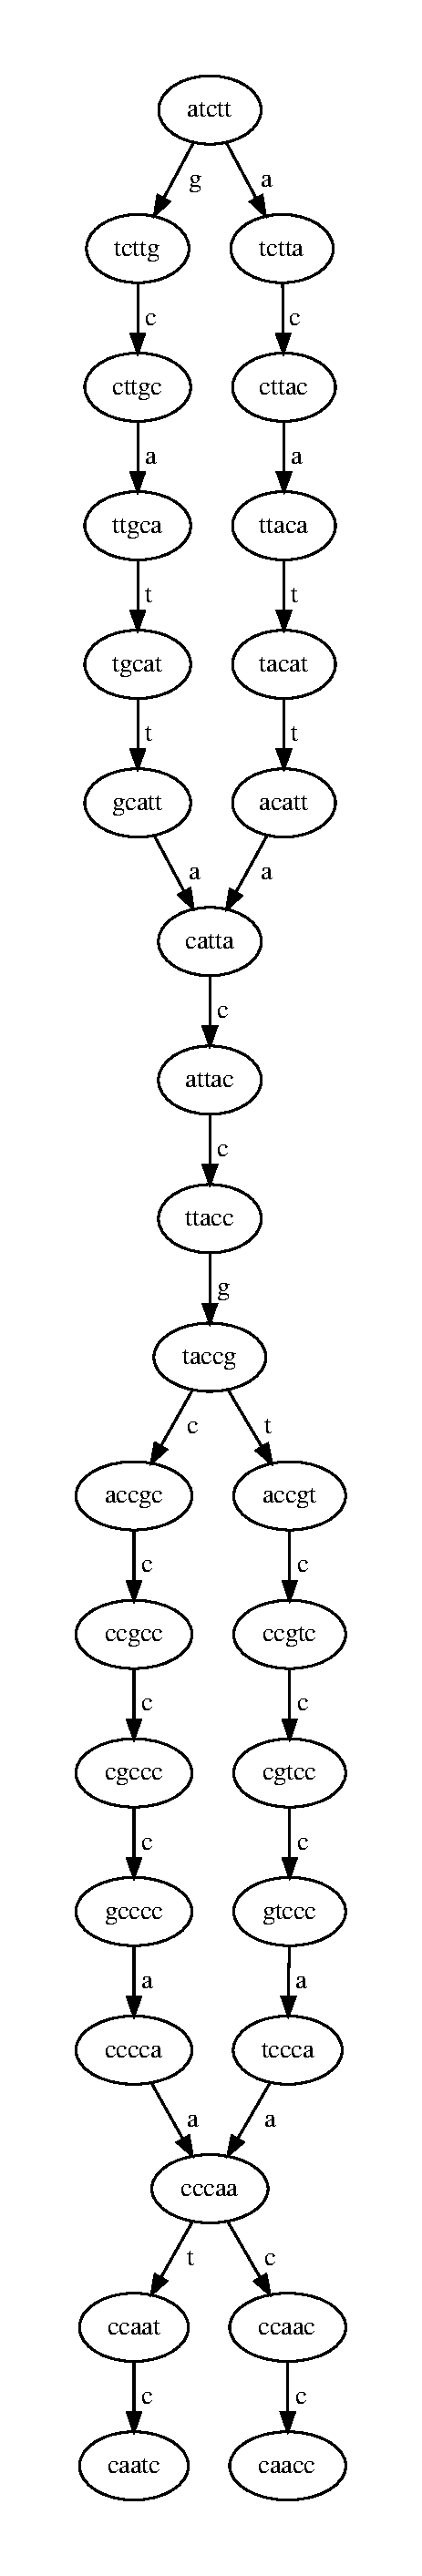
\includegraphics[scale = 0.38]{img/mut.pdf}
  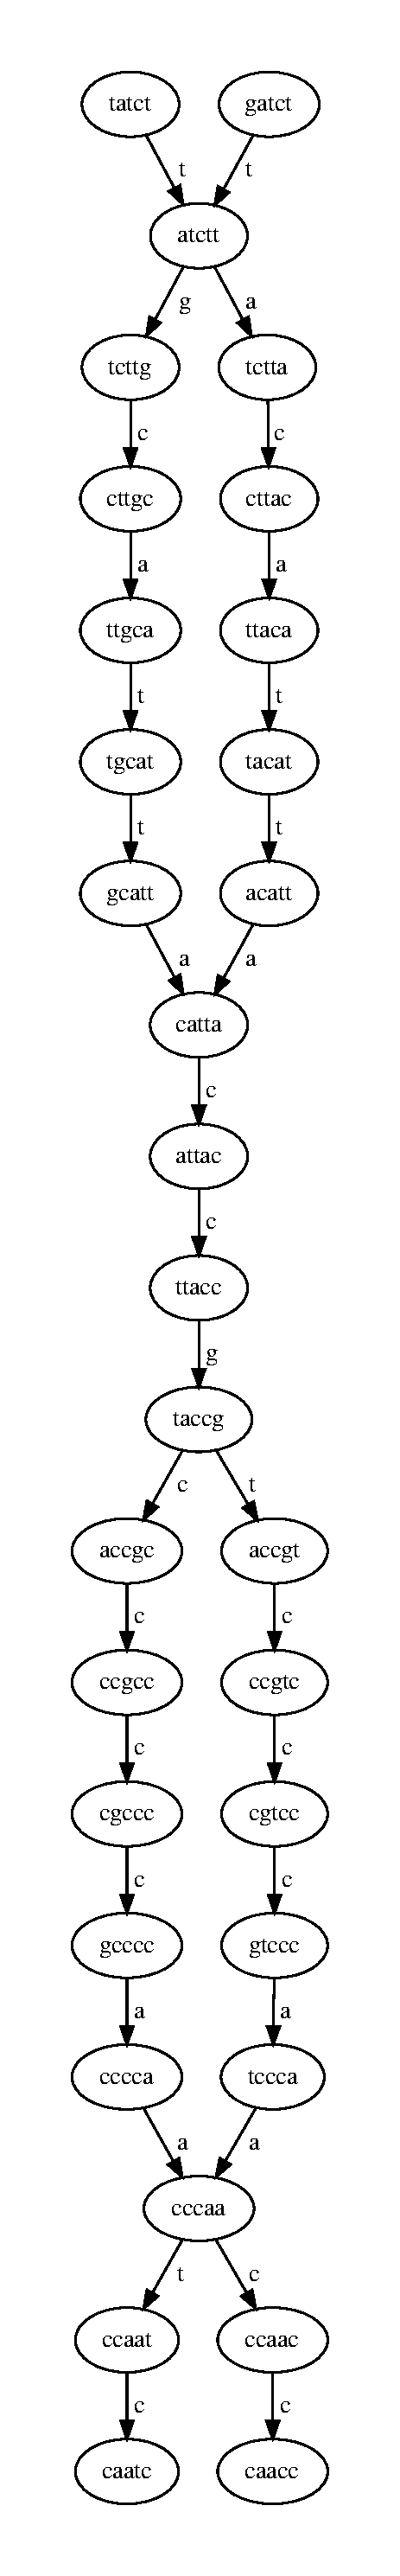
\includegraphics[scale = 0.38]{img/mutns.pdf}
  \caption{Grafi di De Bruijn relativi, rispettivamente, ai due esempi della
    ``versione 1''}
  \label{fig:dbg}
\end{figure}

\noindent
Facciamo le seguenti assunzioni, a livello di pseudocodice, per comodità:
\begin{itemize}
  \item la funzione \texttt{createDBG(v, k)} prende in input un vettore $v$ di
  stringhe e un intero $k$ e restituisce un oggetto rappresentante il
  \textit{grafo di De Bruijn} costruito a  
  partire dalle sequenze contenute in $v$. Tali sequenze sono in questo caso due
  e sono supposte valide secondo le assunzioni fatte all'inizio
  \item si supponga di avere un oggetto \texttt{dbg} rappresentante il
  \textit{grafo di De Bruijn}. Si ha che la funzione \texttt{startNodes(dbg)}
  restituisce un vettore contenente i puntatori ai nodi iniziali/sources, ovvero
  i nodi 
  senza archi entranti del \textit{grafo di De Bruijn}. Per le assunzioni fatte,
  ho almeno un nodo iniziale e al più due nodi iniziali
  \item si supponga che ogni nodo sia rappresentato da un oggetto e che, dato un
  nodo $n$ si abbiano le seguenti funzioni:
  \begin{itemize}
    \item \texttt{label(n)}, che restituisce il \textit{(k-1)-mer} che
    etichetta il nodo $n$
    \item \texttt{outDegree(n)}, che restituisce il numero di archi uscenti dal
    nodo $n$. Se $n==null$ il metodo restituisce comunque 0
    \item \texttt{outLabel(n)}, che restituisce un vettore con le etichette
    degli archi uscenti dal nodo $n$
    \item \texttt{nextNodes(n)}, che fornisce un vettore di puntatori ai nodi
    successivi/figli di $n$
 \end{itemize}
\end{itemize}
\newpage
Vediamo quindi uno pseudocodice possibile per trovare le mutazione usando il
\textit{grafo di De Bruijn}. L'output è dello stesso formato del precedente
algoritmo. 
\begin{algorithm}[H]
  \small
  \begin{algorithmic}[1]
    \Function{CheckMutation}{$seq1$, $seq2$}
    \If{$length(seq1)\neq length(seq2)$}
    \State \textbf{return} $([\,\,\,],\bot)$
    \EndIf
    \If{$length(seq1)==0$ \textbf{or} $length(seq2)==0$}
    \State \textbf{return} $([\,\,\,],\bot)$
    \EndIf
    \State $muts \gets [\,\,\,]$
    \State $seq1\gets lowercase(seq1)$
    \State $seq2\gets lowercase(seq2)$
    \State $i\gets 0$
    \State $dbg\gets createDBG([seq1, seq2], 6)$
    \State $s \gets startNodes(dbg)$
    \If{$length(s) \neq 1$}
    \State $push(muts, newMutation(label(s[0])[0], label(s[1])[0], 0))$ 
    \State $i\gets i+1$
    \EndIf
    \State $curr\gets s[0]$
    \While {$\top$}
    \If{$outDegree(curr) == 2$}
    \State $l\gets outLabel(curr)$
    \State $push(muts, newMutation(l[0],l[1], i+5))$
    \EndIf
    \If{$outdegree(curr) == 0$}
    \State \textbf{break}
    \EndIf
    \State $i\gets i+1$
    \State $curr\gets nextNodes(curr)[0]$
    \EndWhile
    \State \textbf{return} $(muts, \top)$
    \EndFunction
  \end{algorithmic}
  \caption{Algoritmo basato su \textit{kmer} e \textit{grafo di De Bruijn} per
  mutazioni} 
\end{algorithm}
Nel dettaglio, tralasciando quanto uguale alla prima versione:
\begin{itemize}
  \item alla riga 11 si inizializza un indice che tiene conto della posizione
  della mutazione, tramite il numero di nodi del \textit{grafo di De Bruijn}
  visitati 
  \item alla riga 12 si crea il \textit{grafo di De Bruijn} a partire dalla
  coppia di stringhe
  \item alla riga 13 si estrae il vettore di \textit{nodi source}, senza archi
  entranti
  \item alle righe 14-17 si risolve l'assunzione per la quale la prima base può
  subire una mutazione. Qualora non si abbia un solo \textit{nodo source} si
  aggiunge la mutazione che corrisponde ai primi simboli delle etichette di tali
  nodi, che possono essere solo due (non essendo uno) per le assunzioni fatte.
  Si incrementa quindi l'indice 
  \item alla riga 18 si sceglie il primo \textit{nodo source} (unico in assenza
  di mutazione in prima base) come nodo da cui far partire l'iterazione
  \item alle righe 19-31 si studia il grafo
  \item alle righe 20-27 qualora un nodo abbia due archi uscenti, essendo quindi
  in un nodo che inizia una \textbf{bubble}, si aggiunge la
  mutazione corrispondente alle etichette degli archi che portano a tali
  nodi. L'indice di tale mutazione è ottenuto tenendo conto dell'indice
  incrementato di 5, per lo stesso ragionamento della prima versione
  dell'esercizio
  \item alle righe 24-26 si interrompe lo studio del grafo qualora si sia giunti
  ad un \textit{nodo sink}, senza archi uscenti. A questo è possibile solo
  grazie alle assunzioni fatte 
  \item alle righe 27-28 si incrementa l'indice e ci si sposta al nodo
  successivo. Qualora fossimo in un nodo che inizia una \textbf{bubble} si
  sceglie di seguire uno dei due cammini, nel dettaglio il primo
\end{itemize}
\textit{Si noti che senza ulteriori assunzioni si perde esplicita referenza di
quale base della mutazione appartiene alla sequenza di riferimento o a quella
mutata, ma un controllo per capirlo è facilmente eseguibile usando l'indice
della mutazione.}
\begin{esempio}
  Vediamo brevemente un esempio.\\
  Siano date in input:
  \begin{itemize}
    \item atcttgcattaccgccccaatc
    \item atcttacattaccgtcccaacc
  \end{itemize}
  Si costruisce quini il grafo a sinistra della figura \ref{fig:dbg}.\\
  Si parte dal nodo ``atctt''. Si verifica che tale nodo ha due archi uscenti,
  etichettati con ``g'' e ``a''. Si aggiunge quindi la mutazione (che avrà
  indice 5 essendo $i=0$), si incrementa
  l'indice e si prosegue su uno dei due cammini, spostandosi su ``tcttg''. Tale
  nodo ha un solo arco uscente quindi ci si sposta in ``cttgc''. Si
  continua in questa maniera fino a che non si arriva ad un nodo privo di archi
  uscenti. 
\end{esempio}
\section{Versione 3}
Potenzialmente, in fase di creazione del \textit{grafo di De Bruijn}, potremmo
tenere traccia degli archi che ``saltano'' le \textit{bubble}, come in figura
\ref{fig:dbg2}, per poter simulare qualcosa di analogo alla versione 1
dell'algoritmo, evitando di visitare nodi inutili. L'idea è quella di procedere
saltando direttamente dall'inizio di una \textbf{bubble}, dopo aver aggiunto la
mutazione, alla sua fine. \\
Ipotizziamo quindi che, in fase di costruzione del \textit{grafo di De Bruijn},
ogni qual volta si riconosca l'inizio di una \textbf{bubble}, si provveda a
creare, qualora la \textbf{bubble} si chiuda, un arco, di tipologia
diversa rispetto a quelli standard del grafo (anche solo banalmente indicandolo
con 2 anziché 1 nell'ipotetica matrice di adiacenza), che punti alla fine della
\textbf{bubble} stessa. Ipotizziamo quindi l'aggiunta un metodo, dato un
nodo $n$ inizio di una \textbf{bubble} (quindi con \texttt{outDegree(n)==2}),
che chiamiamo
\texttt{toEndBubble(n)}. Tale metodo restituisce il nodo $n'$ di fine
\textbf{bubble} (il primo successivo con due archi entranti). Qualora
\texttt{toEndBubble(n)} restituisca $null$ si ha che la \textbf{bubble} non
viene chiusa prima della fine del grafo, comportando che si è arrivati a fine
computazione.\\  
Il caso di prima base mutata rimane analogo alla versione precedente.\\
Il salto alla fine della \textbf{bubble} implica un comportamento pari a quello
della prima versione dell'esercizio, comportando il medesimo aumento di indice
per poter tener corretta traccia della posizione della mutazione.\\
Possiamo quindi indicare il nuovo pseudocodice dove si vedrà che  la differenza
rispetto alla versione 2 è che, qualora si sia in un 
nodo che inizia una \textbf{bubble}, il nodo seguente, dopo l'aggiunta della
mutazione, non viene scelto come il primo di uno dei due cammini ma, alla riga
26, come il nodo che termina la \textbf{bubble}. L'indice viene incrementato in
riga 27 di conseguenza. In generale si ha quindi un controllo che permette di
capire se si è in un nodo che inizia una \textbf{bubble} o in uno con un solo
nodo successivo e in tal caso si procede normalmente.
\begin{algorithm}[H]
  \small
  \begin{algorithmic}[1]
    \Function{CheckMutation}{$seq1$, $seq2$}
    \If{$length(seq1)\neq length(seq2)$}
    \State \textbf{return} $([\,\,\,],\bot)$
    \EndIf
    \If{$length(seq1)==0$ \textbf{or} $length(seq2)==0$}
    \State \textbf{return} $([\,\,\,],\bot)$
    \EndIf
    \State $muts \gets [\,\,\,]$
    \State $i\gets 0$
    \State $seq1\gets lowercase(seq1)$
    \State $seq2\gets lowercase(seq2)$
    \State $dbg\gets createDBG([seq1, seq2], 6)$
    \State $s \gets startNodes(dbg)$
    \If{$length(s) \neq 1$}
    \State $push(muts, newMutation(label(s[0])[0], label(s[1])[0], 0))$ 
    \State $i\gets i+1$
    \EndIf
    \State $curr\gets s[0]$
    \While {$\top$}
    \If{$outDegree(curr) \neq 2$}
    \State $i\gets i+1$
    \State $curr\gets nextNodes(curr)[0]$
    \Else
    \State $l\gets outLabel(curr)$
    \State $push(muts, newMutation(l[0], l[1], i+5))$
    \State $curr\gets toEndBubble(curr)$
    \State $i\gets i+6$
    \EndIf
    \If{$outDegree(curr)==0$}
    \State \textbf{break}
    \EndIf
    \EndWhile
    \State \textbf{return} $(muts, \top)$
    \EndFunction
  \end{algorithmic}
  \caption{Algoritmo basato su \textit{kmer}, \textit{grafo di De Bruijn} e
  \textit{bubble} per mutazioni} 
\end{algorithm}
\begin{figure}[H]
  \centering
  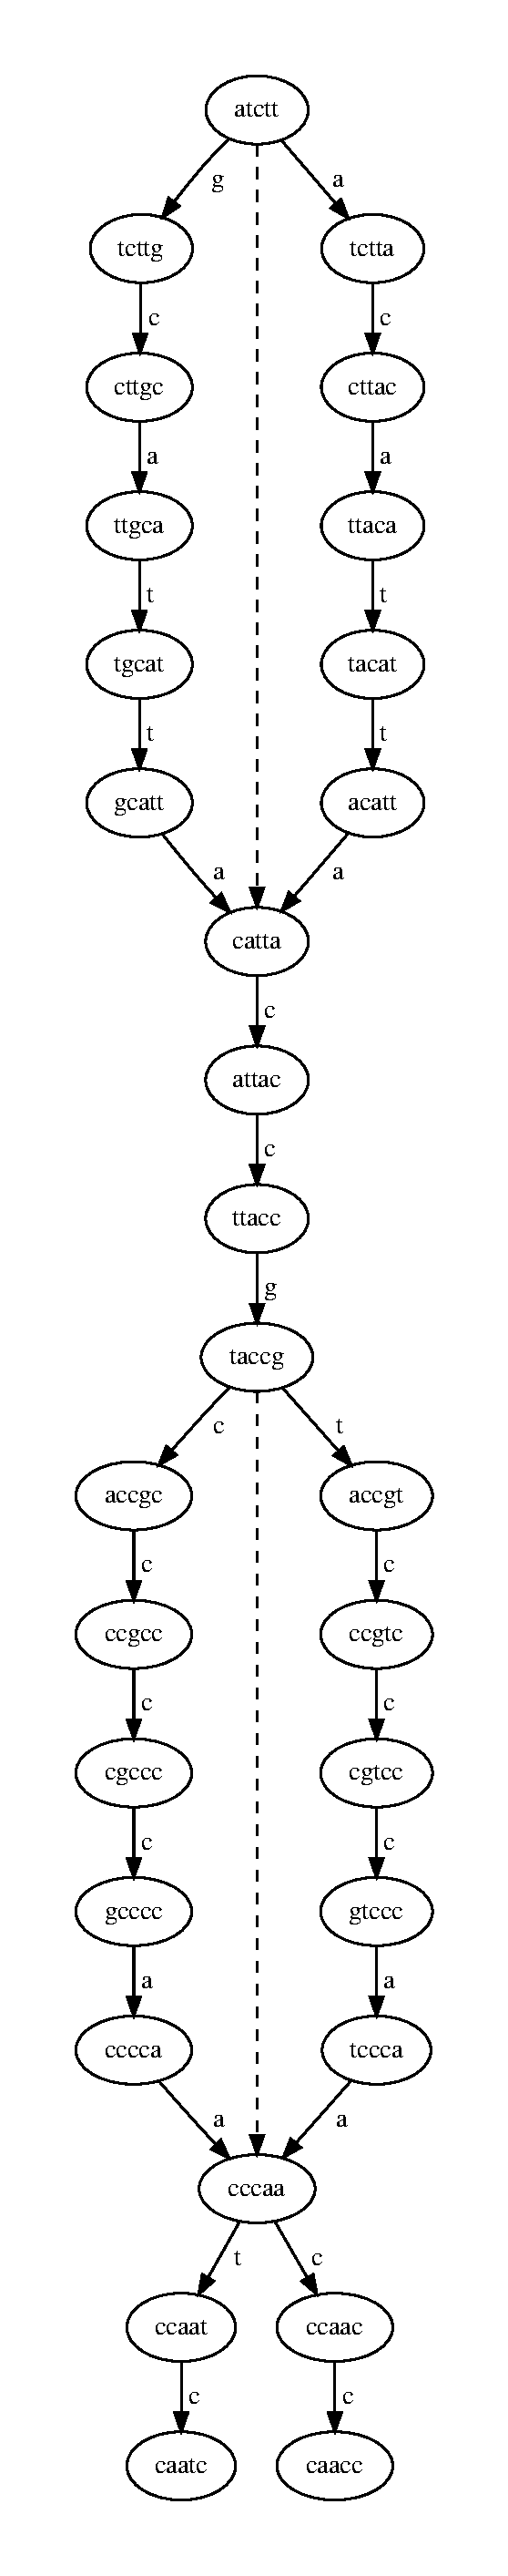
\includegraphics[scale = 0.33]{img/mut2.pdf}
  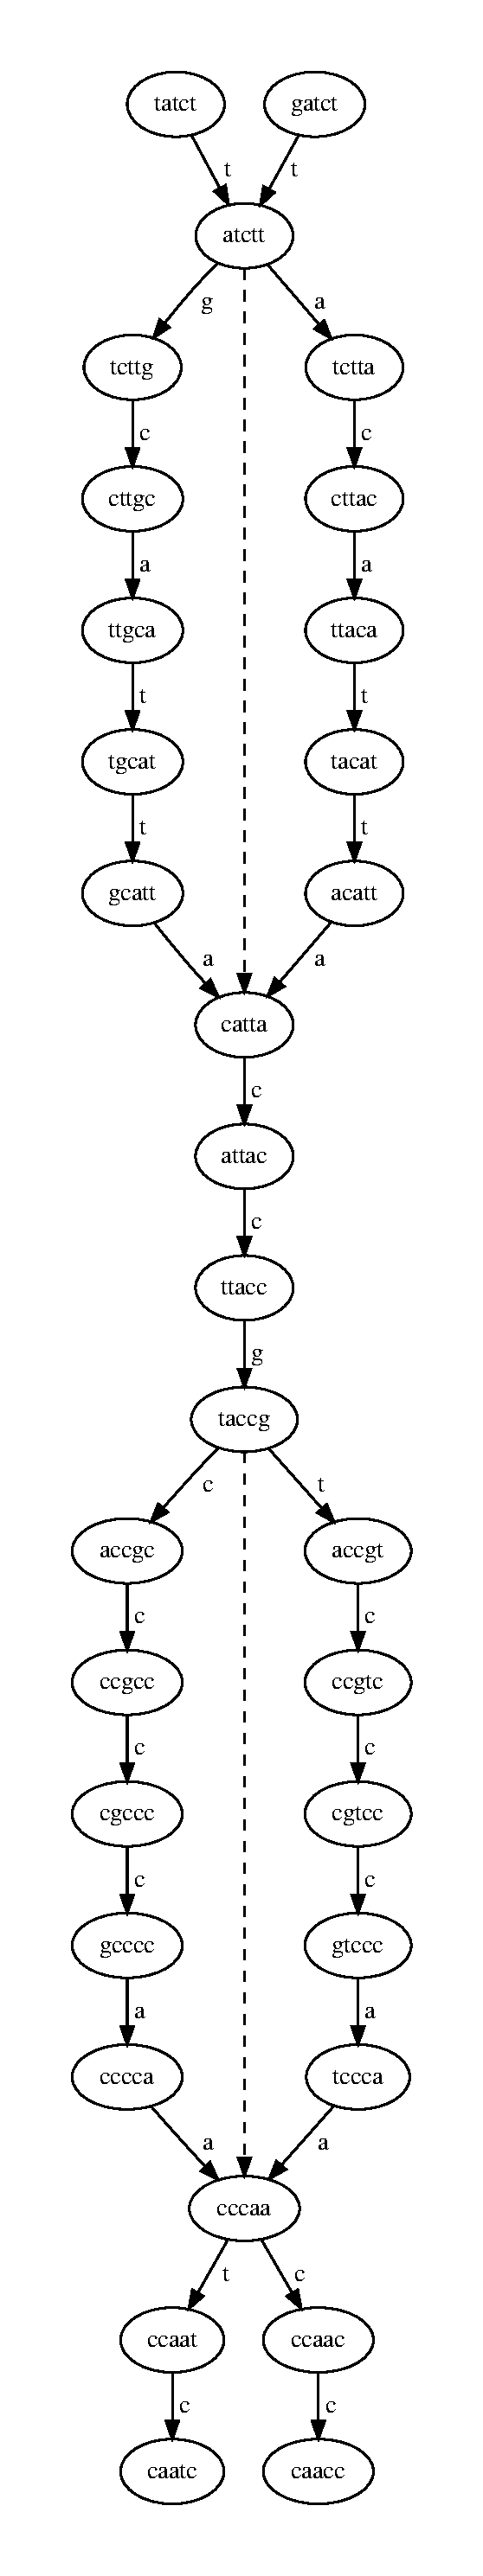
\includegraphics[scale = 0.33]{img/mutns2.pdf}
  \caption{Grafi di De Bruijn relativi con i ``salti'' delle \textbf{bubble},
    rispettivamente, ai due esempi della ``versione 1''}
  \label{fig:dbg2}
\end{figure}
\begin{esempio}
  Vediamo brevemente un esempio.\\
  Siano date le stringhe:
  \begin{itemize}
    \item tatcttgcattaccgccccaatc
    \item gatcttacattaccgtcccaacc
  \end{itemize}
  che sono relative al grafo di destra nella figura \ref{fig:dbg2}.\\
  Si segnala in primis la presenza dei due nodi iniziali ``tatct'' e ``gatct'' e
  quindi si provvede all'aggiunta della mutazione, di indice 0, con ``t'' e
  ``g''. Ci si sposta quindi al nodo ``atctt'', che presenta due archi
  uscenti. Essendo l'indice a 1 si aggiunge la mutazione a indice $1+5=6$ tra
  ``g'' e ``a''. Sfruttando ora il ``salto'' della \textbf{bubble} ci si sposta
  al nodo ``catta''. Tale nodo presenta un solo arco uscente e quindi di
  prosegue passando al nodo ``attac''. Si prosegue così fino ad arrivare ad un
  nodo privo di archi uscenti, concludendo la computazione.
\end{esempio}
\noindent
Le due versioni coi \textit{grafi di De Bruijn} sono state studiate per
curiosità e per capire meglio la struttura, dal punto di vista didattico. Nel
dettaglio, per questo problema, 
date le assunzioni, il calcolo del grafo comporta un costo computazionale
aggiuntivo che risulta essere però superfluo.

\chapter{Esercizio 3}
La \textbf{distanza di Hamming} tra due stringhe, che si assumono di uguale
lunghezza, è 
il numero di indici per i quali i due caratteri associati sulle due stringhe
sono diversi. È quindi un conteggio delle sostituzioni necessarie per passare da
una stringa all'altra.\\
Ipotizzando di voler studiare la distanza di Hamming tra due sequenze tramite la
griglia estesa si può ipotizzare di ragionare solo in termini di una delle due
sequenze, ovvero considerare i pesi degli archi in ottica di una sola delle due
sequenze. Si associano quindi i seguenti pesi, come in figura \ref{fig:pes3}:
\begin{itemize}
  \item $w(diagonale)=0$
  \item $w(verticale)=0$
  \item $w(orizzontale)=1$
\end{itemize}
o, in modo speculare se si vuole ragionare sull'altra sequenza:
\begin{itemize}
  \item $w(diagonale)=0$
  \item $w(verticale)=1$
  \item $w(orizzontale)=0$
\end{itemize}
\begin{figure}
  \centering
  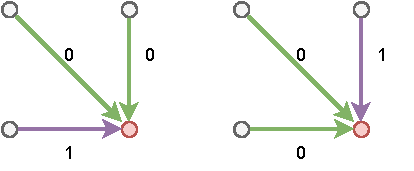
\includegraphics[scale = 1.3]{img/es31.pdf}
  \caption{Rappresentazione grafica dei pesi degli archi.}
  \label{fig:pes3}
\end{figure}
Dove, in entrambi i casi, gli archi diagonali rappresentano un match mentre, a
seconda, gli archi verticali o quelli orizzontali tengono conto dei mismatch.\\
A questo punto si cerca il cammino di peso minimo che parte dal nodo
\textit{source}, posto in alto a sinistra, e arriva al nodo \textit{sink}, posto
in basso a destra. Essendo il nodo sink in posizione $(n,n)$, assumendo le due 
sequenze lunghe $n$, garantisco che, calcolando il cammino che parte dal nodo
source $(0,0)$ e arriva in quel nodo, si abbia il valore della
distanza di Hamming, che prevede stringhe di ugual lunghezza. I vari valori
degli altri nodi sono da considerarsi ``temporanei'' e non rappresentanti una
distanza di Hamming. Potenzialmente però tutti e soli i nodi $(i,i)$, con
$i\in[1,n)$, oltre quindi al nodo sink, potrebbero essere i nodi di fine di
potenziali cammini dal source per calcolare la distanza di Hamming tra le
sottostringhe di lunghezza $i$ delle due stringhe in input.\\
\begin{esempio}
  Prendendo, ad esempio, in input:
  \begin{itemize}
    \item AAAGTTC
    \item AAACTTT
  \end{itemize}
  Si ha un cammino minimo (non l'unico), assumendo costo degli archi in
  orizzontale pari a 1 e in verticale pari a 0, del tipo:
  \begin{figure}[H]
    \centering
    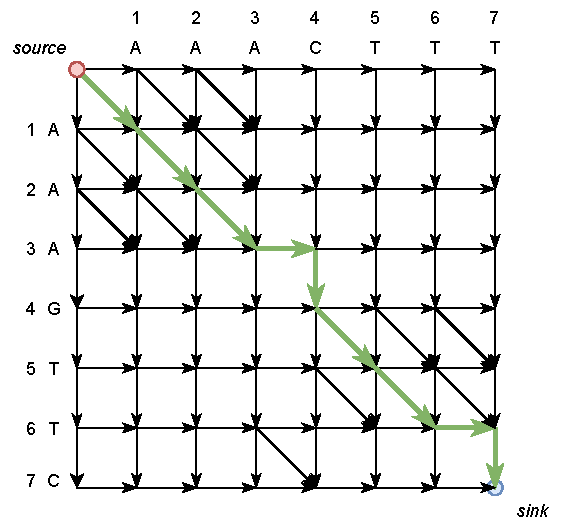
\includegraphics[scale = 1]{img/es3.pdf}
  \end{figure}
  \noindent
  Dove in verde è segnato il cammino minimo scelto. Avendo solo due archi
  orizzontali, che ricordiamo avere peso 1 mentre gli altri hanno peso nullo,
  possiamo concludere che la distanza di Hamming tra le due stringhe è 
  pari a 2.\\
  Per il ragionamento fatto sopra, se mi fermassi in $(3,3)$, per $i=3$, avrei
  la distanza di Hamming tra AAA e AAA. Il cammino dal source a $(3,3)$ è
  formato da sole diagonali e quindi ha costo 0, che è appunto al distanza di
  Hamming tra le due sottostringhe.
\end{esempio}
\chapter{Esercizio 4}
Il problema della \textbf{longest common substring} si pone l'obiettivo di
estrarre, a partire da due stringhe di lunghezza arbitraria, anche non uguale,
la sottostringa, comune ad entrambe, più lunga.\\
Dal punto di vista della griglia si assegnano i seguenti pesi (come da figura
\ref{fig:pes4}): 
\begin{itemize}
  \item $w(diagonale)=1$
  \item $w(verticale)=-i$
  \item $w(orizzontale)=-j$
\end{itemize}
\begin{figure}
  \centering
  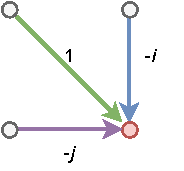
\includegraphics[scale = 1.3]{img/es41.pdf}
  \caption{Rappresentazione grafica dei pesi degli archi. Si ricorda che nel
    nodo finale, in rosso,
    posso comunque avere solo valori $\geq 0$}
  \label{fig:pes4}
\end{figure}
Dove gli archi diagonali rappresentano un match ed $i$ e $j$ sono gli indici che
scorrono le due stringhe, ovvero rispettivamente sulle righe e sulle colonne.\\
Si assume che i nodi abbiano valore $x\geq 0$ quindi
\textbf{qualora si ottenga un valore negativo come risultato dopo
  l'attraversamento dell'arco viene messo il valore 0}.\\
Quando si ha un match quindi il nodo finale ha valore pari a uno più il valore
del nodo sorgente dell'arco diagonale.\\
Si ragiona quindi tenendo traccia del valore massimo raggiungo, tenendo traccia,
per una maggior efficienza, anche delle coordinate. Una volta completata la
griglia si avrà che il valore massimo corrisponde al nodo \textit{sink} del
cammino composto dalla più lunga sequenza possibile di archi diagonali
consecutivi. Qualsiasi altra ``operazione'', con archi orizzontali o diagonali,
comporta infatti una perdita di punteggio e ogni volta che un cammino diagonale
termina viene azzerato il punteggio, tramite pesi negativi pesati sugli
indici. Azzerando ogni volta si permette di avere la costruzione di un eventuale
cammino diagonale che assegna man mano il valore corrispondente alla lunghezza
del cammino stesso, avendo che la diagonale pesa 1. Il valore massimo quindi
altro non è che  
la lunghezza della \textit{longest common substring}. Sapendo che archi
diagonali corrispondono a match tra le due sequenze si ottiene che tale cammino
corrisponde alla \textit{longest common substring}. \\
Volendo si può scegliere di salvare in un vettore i valori massimi qualora
coincidano, per ottenere eventuali più \textit{longest common substring} qualora
ce ne siano.\\
In altri termini si cerca il sottocammino più pesante.\\
ipotizzando di non ``azzerare'' ogni volta in caso di mismatch otterrei comunque
una griglia dover il nodo massimo mi permetterebbe di risalire la diagonale
ritrovando la \textit{longest common substring} ma tale nodo non potrebbe avere
come valore la lunghezza della stessa, in quanto non ricomincerei il conto da 0
ogni volta che creo un nuovo cammino fatto di diagonali.
Per ricostruire la \textit{longest common substring} si parte dal nodo
\textit{sink}, come detto definito dal valore massimo calcolato. Si aggiunge il
carattere corrispondente e si risale tutto il cammino diagonale, aggiungendo di
volta in volta in testa il carattere letto. Ci si ferma quindi quando non si ha
più un nodo il cui punteggio è stato ottenuto tramite un arco diagonale.
\begin{esempio}
  Vediamo quindi un esempio pratico. Siano date:
  \begin{itemize}
    \item AAACGCGCTTTTTCCCAT
    \item AAAGGGGCGCGCTTTTTAAA
  \end{itemize}
  \newpage
  Si costruisce quindi la griglia e si identifica il cammino diagonale più
  lungo: 
  \begin{figure}[H]
    \centering
    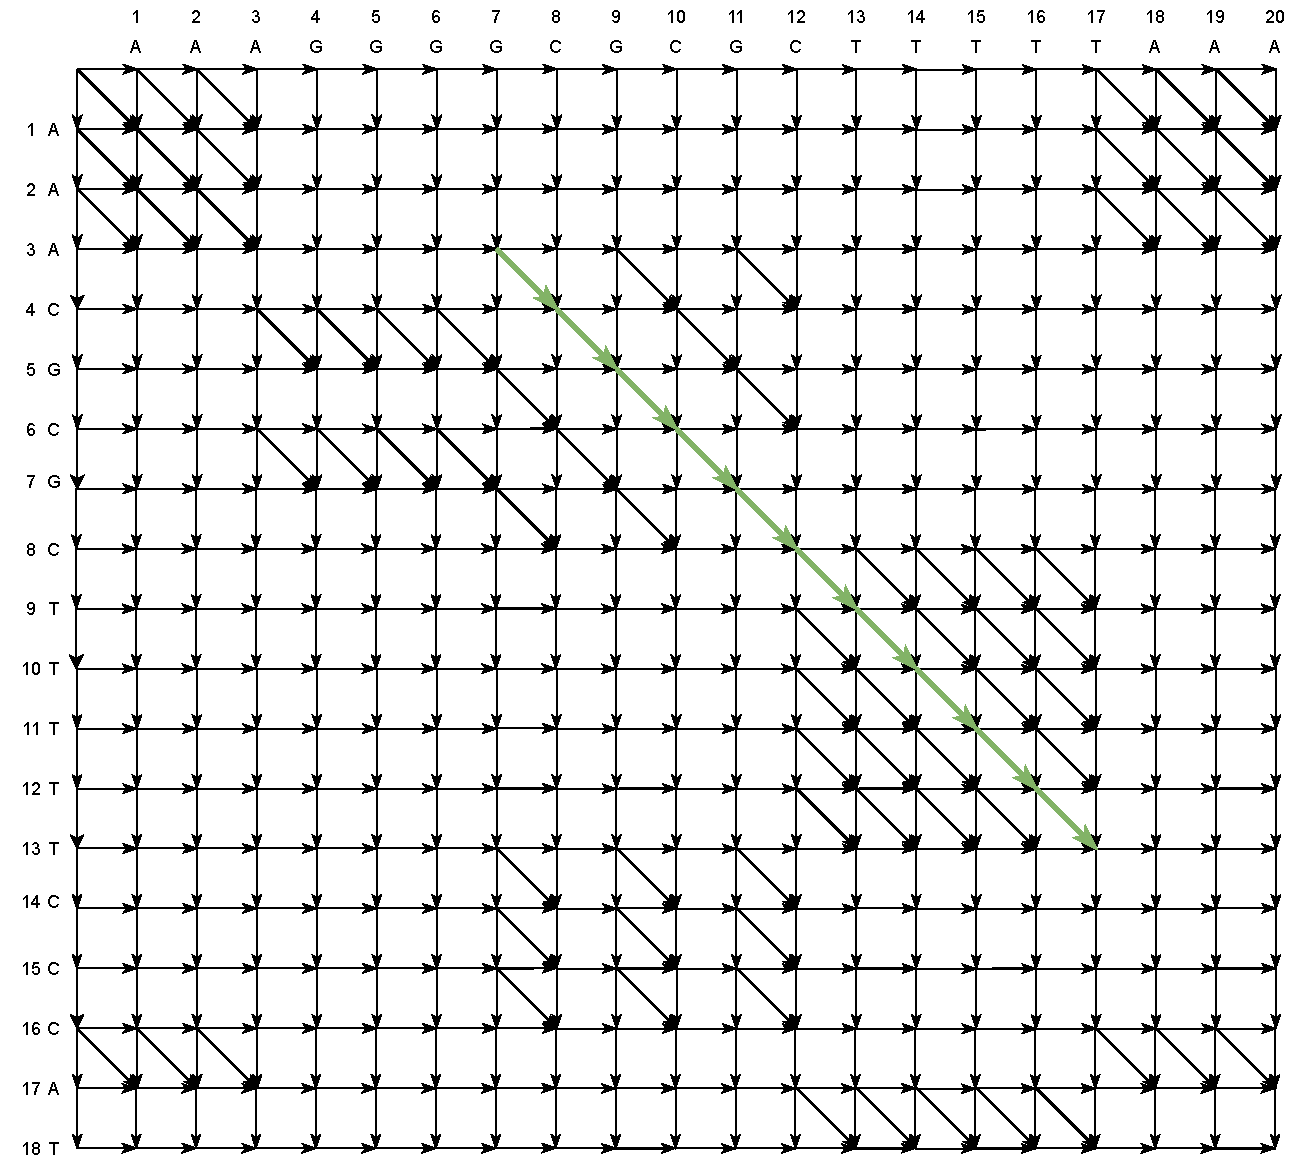
\includegraphics[scale = 0.62]{img/es4.pdf}
  \end{figure}
  Ricostruendo si ha che tale cammino identifica un massimo pari a 10. Il
  sottocammino più pesante è quindi quello rappresentato in verde. Ipotizzando
  quindi di poter `risalire'' la dialogale si
  ricostruisce: 
  \begin{center}
    CGCGCTTTTT
  \end{center}
  che è appunto la \textit{longest common substring} delle due sequenze in
  input. 
\end{esempio}
\chapter{Link al codice}
Durante lo svolgimento dell'assignment è stato elaborato anche il codice in
\textit{Rust} per i vari esercizi, con i vari unit test correlati. In merito al
codice relativo ai grafi di De Bruijn si specifica che alcuni metodi sono
possibili solo grazie alle assunzioni fatte in merito all'esercizio 2.\\
Il codice, insieme al \TeX\,  di questa relazione, è disponibile nella
repository (a partire dalla data di scadenza dell'assignment):
\url{https://github.com/dlcgold/es_bio}.\\ 
\\
Per eseguire i test:
\begin{shaded}
  \noindent
  \texttt{> cd 1/esbio}\\
  \texttt{> cargo test}
\end{shaded}
\noindent
Per eseguire i test con alcune stampe:
\begin{shaded}
  \noindent
  \texttt{> cd 1/esbio}\\
  \texttt{> cargo test -- --nocapture}
\end{shaded}
\noindent
Per visualizzare la piccola documentazione:
\begin{shaded}
  \noindent
  \texttt{> cd 1/esbio}\\
  \texttt{> cargo doc --open}
\end{shaded}
\end{document}
% LocalWords:  sottostringhe sottostringa pseudocodice lowercase Hamming
